\chapter{コンポーネントの作成}

ドメインの表現、集計データの作成、関数によるデータ変換、状態の作成、並行処理の使用など、基礎は固まりました。次は、より大きな単位で、問題に対応するコードの構築を始める番です。この大きな単位をコンポーネントと呼ぶことにします。コードをコンポーネントに分割することで、問題に対応する部分をより高いレベルで考えることができるようになります。また、コンポーネントの境界は、複数の開発者やチームにコードベースを分割するのに適した方法です。また、再利用の機会にもなり得ます。

コンポーネントは、より細かい要素(関数、レコード、プロトコル)の集合体であり、全体として大きな目的を持っている。呼び出し元が使用する外部APIを備えている。また、コンポーネントの状態を含む内部実装を持ち、内部で並行処理を行い、データを並列処理したり、イベントに対応するための別スレッドを作成したりすることもできます。

アプリケーションの機能をClojure名前空間に整理する方法を見て、コンポーネントの考察を開始します。これは、コンポーネントの内部と外部の両方を含むすべてのコードに適用されます。次に、呼び出し元が使用する外部APIについて見ていきます。これは、関数呼び出しインターフェースと、より長寿命の \texttt{core.async} チャンネルの使用の両方を考慮する必要があります。最後に、コンポーネントの内部をどのように実装するか、状態や並行性のために既に見たツールを使ってコンポーネントの状態やそのライフサイクルを管理するかについて見ていきます。

第7章「アプリケーションを構成する」では、これらのコンポーネントを次のステップとして、アプリケーションを完全に組み立てていきます。


\section{名前空間による整理}

Clojureコードは、一連の個々のトップレベル・フォーム(関数、レコード、プロトコルなど)としてコンパイルされ評価されますが、Clojureはそれらの個々のフォームをグループ化するための名前空間を提供します。名前空間は、フォームのグループを収集し、整理し、名前を付けるために使用できる、名前付きの階層的なコンテナです。名前空間の実用的な使い方の1つは、どこかで同じ名前と衝突することを心配することなく、コードで単純な名前を使えるようにすることです。名前空間は、どれを意味しているのかを指定する手段を提供します。

Clojureのコードはより細かい要素で構成されていますが、依存関係は関数レベルではなく、名前空間レベルで宣言され、読み込まれます。各名前空間の \texttt{ns} マクロは、その依存関係を定義し、まとめて依存関係グラフを作成する。この依存関係グラフは、名前空間がロードされる順序に影響を与える。名前空間がマルチメソッドやプロトコル(いずれも型固有の動作のためのオープンシステム)の実装を提供する場合、実装を使用する前にロードする必要があるため、このロード順序が重要になることがあります。

名前空間とコンポーネントは、どちらも組織化のためのツールである。名前空間は機能を整理するための言語機能であり、コンポーネントは問題レベルで整理するための手段である。この2つのアプローチは、どちらも有用であり、連動してコードを構造化し、最終的に他の開発者が理解しやすく、使いやすくするものです。

\subsection{名前空間のカテゴリ}

Clojureで関数のセットを名前空間にグループ化するのは、多くの理由があります。以下のカテゴリは、アプリケーションを反映した論理的な名前空間アーキテクチャを作成するために使用することができます。

\begin{description}
\item [Utility] utility名前空間は、ドメインや目的別に整理された汎用的な関数を提供します。例えば、文字列操作や特定のファイル形式の解析のための名前空間を作成することができます。一般に、utility名前空間は依存関係がほとんどありません。
\item [Data definition] カスタムコレクションやドメインエンティティのセットを、コレクションやエンティティを使用するためのヘルパー関数と一緒にネームスペースで定義するのが一般的である。
\item [Abstraction] プロトコルのような抽象的なものは、最小限の依存関係でネームスペースに分離することができます。
\item [Implementation] 一方、プロトコルやインタフェースで定義された抽象化機能を名前空間で実装すると便利なことが多い。この実装は、アプリケーションに組み入れることができる。
\item [Assembly] 実装のセットと、実装をどのように構築し接続するかを指定する構成がある場合、assembly名前空間がすべてを結びつけます。実装の内部では、一般に抽象化(プロトコル)またはデータ構造のみが直接使用される。
\item [Entry point] ほとんどのアプリケーションには、アプリケーションの開始(設定の収集を含む)とアセンブリや他のライフサイクル操作の開始をつなぐ1つ以上のエントリーポイントがあります。
\end{description}

次の図は、ライブラリやアプリケーションの中で、これらの種類の名前空間がどのように一般的に重なり合っているかを示しています。

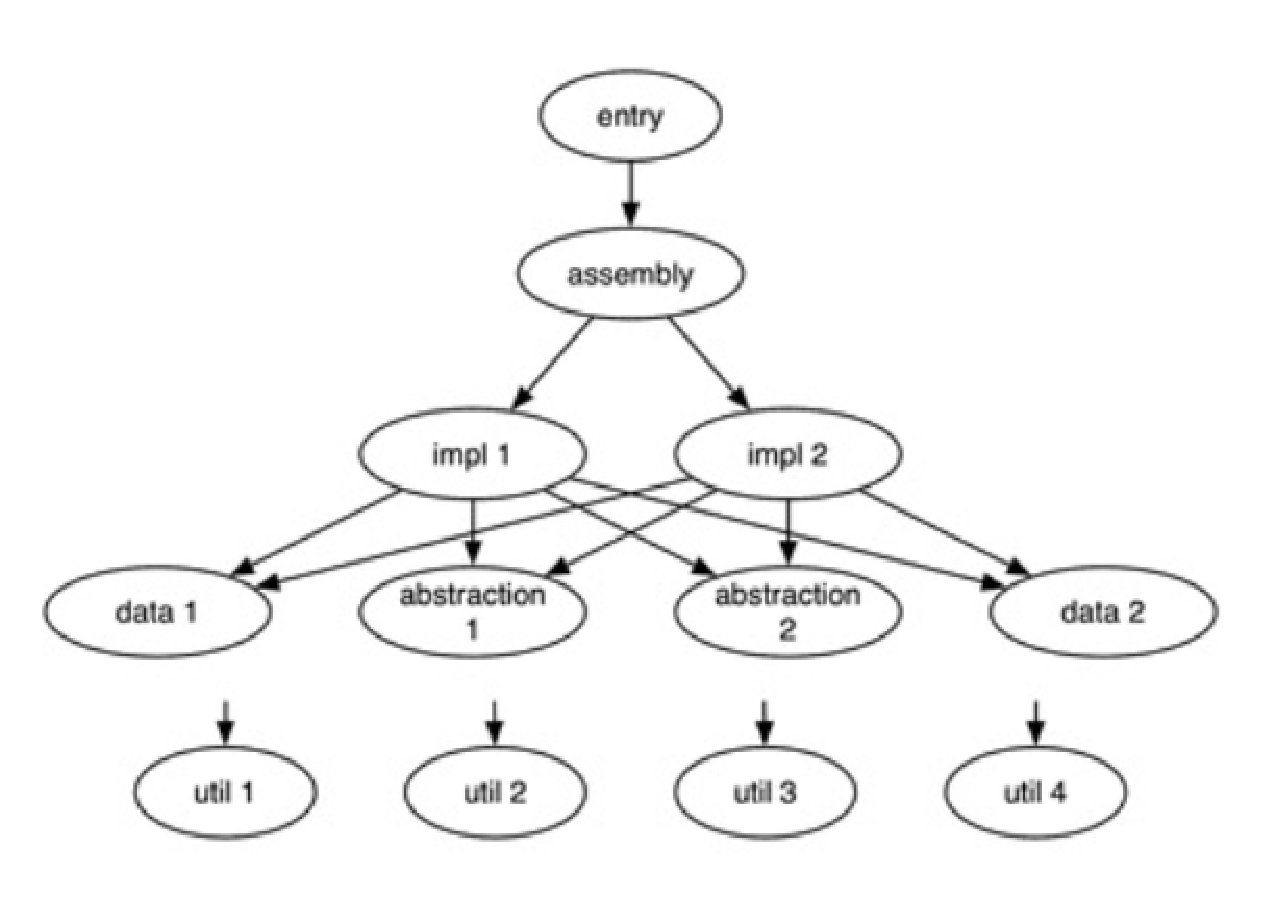
\includegraphics[width=10cm]{fig_06_001.eps}

この構造は、独自の名前空間構造を設計する際のガイドラインとして有効である。ユーティリティ名前空間は依存関係グラフの一番下にあり、それ自身の依存関係はほとんどなく、上の複数の名前空間によって使用されています。次の層は、データまたは抽象化名前空間のいずれかからなり、アプリケーション自体のビルディングブロックを作成します。抽象化の上には、その抽象化のための実装があります。その上には、設定が処理され、実装が組み立てられて接続され、 アプリケーションの状態が作成されるアセンブリ層があります。一番上には、ウェブアプリケーション、コマンドラインインターフェース、サービスなど、一つまたは複数のエントリーポイントがあります。

プロジェクト内の名前空間を名前空間ツリーとして整理するには、さまざまなアプローチがありますが、唯一の正解はありません。小規模なプロジェクトでは、ネームスペースの大部分をプロジェクトにちなんだ単一のルート内に配置し、ネストを最小限にすることがよくあります。

\begin{lstlisting}[numbers=none]
myproject.util.string ;; utility
myproject.util.json ;; utility
myproject.domain    ;; data - domain entities
myproject.config    ;; data - config data
myproject.services  ;; abstraction - service definitions
myproject.impl.xyz  ;; implementation of service abstraction
myproject.assembly  ;; assembly
myproject.main      ;; main entry point - command-line
\end{lstlisting}

小規模なシステムでは、多くの抽象化機能、実装、ユーティリティをグループ化して、サービスを水平方向に切り分けるのが最も簡単な場合があります。システムが大きくなるにつれて、システムを縦割りにして、それぞれのコンポーネントをAPI、実装、データ定義のセット、ユーティリティで構成することがますます有用になってきます。

\subsection{パブリックとプライベートの関数}

Clojureは、データや関数をデフォルトで利用できるようにすることに偏っています。しかし、ほとんどの名前空間には、ヘルパーとして使用される関数や、決して一般的な使用方法の一部となることを意図していない関数があります。名前空間内の関数を定義するときは、消費者がそれらの関数をどのように認識し、どのように使用することが期待されるかを考えてください。いくつかのツールや規約は、プライベートvar、ドキュメント文字列、そして名前空間の構造そのものです。

Clojureに組み込まれた主要なツールは、 \texttt{defn-} または \texttt{\^:private} メタタグを使用して関数をプライベートとしてマークする機能です。


\begin{lstlisting}[numbers=none]
(defn- internal-function [] ...)
(def ^:private internal-constant 42)
\end{lstlisting}


これらのvarはいくつかの名前空間関数の結果から省略されますが、それでもreader var構文で直接アクセスしたり、名前空間オブジェクトを直接呼び出したりすることは可能です。

autodocのようなドキュメント生成ツールは、docstringを持たない関数を省略することがあります。Clojureコア自身は、高度なClojure開発には有用ですが、一般的な使用には適さない内部関数を強調しないためにこの機能を使用します。

最後に、 \texttt{myproject.internal.db} のような名前空間を使用して、内部であることを明示的にマークするのはよくあることで、 \texttt{internal} 以下のすべての名前空間は非パブリックとみなされます。

これらのテクニックは、自分のコードの利用者にどこから手をつければよいかを示すのに役立つと思われます。

さて、名前空間をどのように整理すればいいのかがわかったところで、 それらの名前空間を使っていくつかのコンポーネントを作成してみましょう。まずはコンポーネントのAPIをどのように設計するかを考えてから、コンポーネントをどのように実装するかを考えていきます。






 % Organizing with Namespaces
\section{コンポーネントAPIの設計}

アプリケーション内でコンポーネントを特定する場合、そのコンポーネントがどのような目的を持ち、他のコンポーネントからどのように使用されるかを考えることから始める必要があります。代表的なコンポーネントには、情報管理、プロセッサ、ファサードなどがあります。情報マネージャーは、メモリ内または外部のデータストアにある状態を追跡し、データの作成、変更、問い合わせの操作を提供します。プロセッサーは、データの変換や計算を行うコンポーネントである。ファサードコンポーネントは、主に別の外部システムにアクセスできるようにする(プラグイン可能な)ために存在します。

実際には、ほとんどのコンポーネントはこれらの箱にきれいに収まるわけではなく、1つまたは複数の側面を組み合わせて、独自のアプリケーションのユニークなニーズを満たすコンポーネントにします。

コンポーネントを設計する際に最初に考慮すべきことは、外部の消費者が使用するAPIです。コンポーネントとの対話には、主に2つの方法があります。関数を呼び出す方法と、キューやチャネルでメッセージを渡す方法です。まず、関数について見てみましょう。

\subsection{関数によるコンポーネントデータの操作}

API関数は、外部の消費者がコンポーネントと対話できるようにするための、ノブ、ボタン、またはゲージのようなものです。Clojureでは、多くのものがユーザーによって関数として呼び出されますが、関数、マクロ、プロトコル、マルチメソッドなど、異なる実装があります。(他のもの-マップ、セット、キーワード、シンボルなど-はAPIの一部としてあまり有用ではありません)。

コンポーネントレベルに焦点を合わせましたが、これまで学習したことをすべて覚えておく必要があります。可能な限り、コンポーネントはイミュータブルなデータを直接公開すべきです。イミュータブルであるため、コンポーネントのデータの一部をコンシューマーに渡しても害はありません:コピーは必要ありませんし、コンポーネント自身のデータが影響を受けることもありません。呼び出し元がデータを手に入れたら、自由にClojureツールを使ってクエリや変換を行うことができます。

リクエストを受け取り、自動応答を形成するために使用されるルールのセットを管理する知識エンジンのコンポーネントを考えてみましょう。ルールの具体的なフォーマットはひとまず置いておいて、各ルールがデータとして定義されていると仮定します。ルールを追加、置換、削除するためのAPI関数と、何らかの基準に基づいてルールを検索するための関数が必要です。また、ルールを起動し、手元の作業を行うための関数も必要である。

\begin{lstlisting}[numbers=none]
;; 注:keはステートフル知識エンジン・コンポーネントを指す
;; Read interface
(defn get-rules [ke])
(defn find-rules [ke criteria])
;; Update interface
(defn add-rule [ke rule])
(defn replace-rule [ke old-rule new-rule])
(defn delete-rule [ke rule])
;; Processing interface
(defn fire-rules [ke request])
\end{lstlisting}

そして、これらの関数を次のように使うことができる。

\begin{lstlisting}[numbers=none]
(defn example [] (let [ke (new-ke)]
    (add-rule ke :r1)
    (add-rule ke :r2)
    (add-rule ke :r3)
    (replace-rule ke :r1 :r1b)
    (delete-rule ke :r3)
    (get-rules ke)))
\end{lstlisting}

しかし、もう少し深く見てみると、より小さな関数の集合でAPI全体をサポートできることがわかります。

\begin{lstlisting}[numbers=none]
;; Get the rule-set
(defn get-rules [ke])
;; Transform from one rule-set to another
(defn transform-rules [ke update-fn])
;; Produce a response from a request
(defn fire-rules [ke request])
\end{lstlisting}

\texttt{find-rules}関数は\texttt{get-rules}に対するフィルタリングとして実装することができる.\texttt{add-rule}、\texttt{replace-rule}、\texttt{delete-rule}関数はすべて、ルールセット全体に対する\texttt{transform-rules}の適用と見なすことができる。

ほとんどのAPIはこのパターンを持っている。つまり、少数の重要な基本関数と、使いやすさのために提供されるより大きな関数群である。プロトコルは、複数の実装がそのプロトコルを拡張できるように、機能の中核となるセットを捕捉する良い方法である。派生機能はAPIネームスペースで提供され、プロトコルの上にレイヤー化されるべきである。API関数は、プロトコルを拡張するあらゆるエンティティで動作する。

これを完全な名前空間にまとめると、次のようになる。

\begin{lstlisting}[numbers=none]
(ns components.ke)

;; SPI protocol
(defprotocol KE
  (get-rules [ke] "Get full rule set")
  (transform-rules [ke update-fn]
    "Apply transformation function to rule set. Return new KE.")
  (fire-rules [ke request]
    "Fire the rules against the request and return a response"))

;; private helper functions
(defn- transform-criteria [criteria]
  ;; ...
  )

;; api fns built over the protocol
(defn find-rules
  [ke criteria]
  (filter (transform-criteria criteria) (get-rules ke)))

(defn add-rule
  [ke rule]
  (transform-rules ke #(conj % rule)))

(defn replace-rule
  [ke old-rule new-rule]
  (transform-rules ke #(-> % (disj old-rule) (conj new-rule))))

(defn delete-rule
  [ke rule]
  (transform-rules ke #(-> % (disj rule))))
\end{lstlisting}

この実装では、図にあるように、小さな拡張可能な抽象化(サービスプロバイダインタフェース)の上にコンポーネントAPIを重ねる形で定義しています。

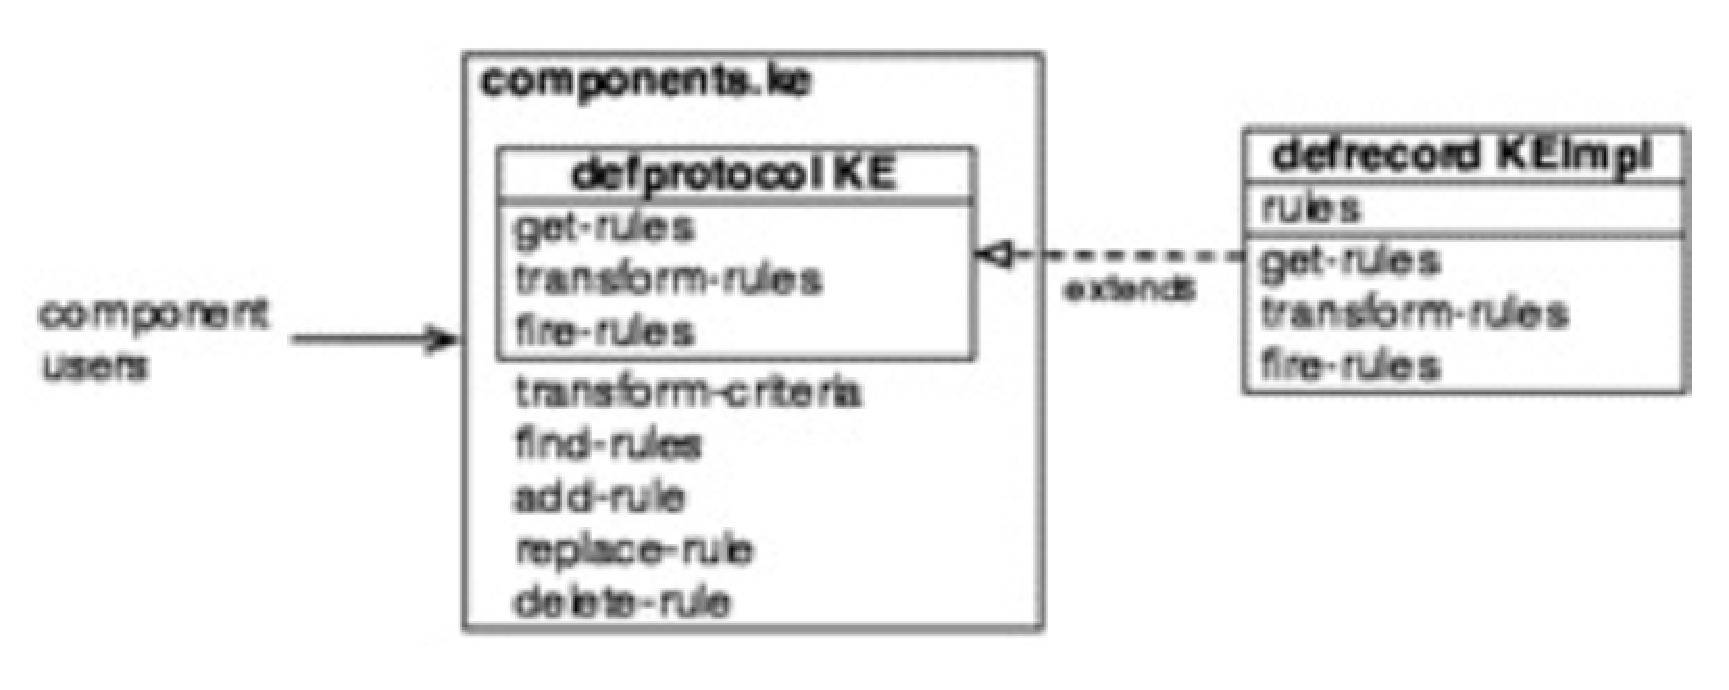
\includegraphics[width=10cm]{fig_06_002.eps}

API全体のプロトコルを作成すると、どのような実装でもすべての関数を再実装する必要があります。その代わり、Clojureで関連する関数のセットを収集するための最適なツールは、プロトコルではなく名前空間です。プロトコルは、今回のように拡張のための最小限の抽象化を定義しているときに最適です。

このコンポーネントの状態実装部分については後で説明し、今は非同期呼び出しなど、他のAPIに関する考察に焦点を合わせます。


\subsection{非同期API}

第5章「コアを使う」では、非同期API関数に対して1回限りの非同期応答を提供するためのfuturesやpromiseといったツールについて既に説明しました。前のセクションで出てきた \texttt{fire-rules} 関数を考えてみましょう。レスポンスを生成するのに時間がかかるかもしれないので、呼び出し元をブロックするのではなく、futureを返すこともできます。

\begin{lstlisting}[numbers=none]
  (let [response-future (fire-rules ke request)]
    ;; ... other work...
    @response-future) ;; レスポンスを取得するために参照する
\end{lstlisting}

応答のためにブロックするのではなく、futureを返すことで、呼び出し側がブロックするタイミングを選択できる(futureをdereferencingすることで)。もう一つの選択肢は、ここに示すように、コールバックを受け取るか(関数を呼び出す)、プロミスを返すか(結果を提供する)である。


\begin{lstlisting}[numbers=none]
;; 知識エンジンが起動するfire-rulesにコールバックを送る。
(let [callback (fn [response] ...)]
  (fire-rules ke request callback))

  ;; 知識エンジンが応答を返すために使うpromiseを送る
(let [result-promise (fire-rules ke request)]
  ;; 必要なときにresult-promiseを参照する。
  @result-promise)
\end{lstlisting}

非同期API呼び出しにどちらが適しているかは、APIそのものよりも呼び出し側のコードに依存します。

さて、直接または非同期の関数呼び出しでAPIを作成する方法を見てきましたが、アプリケーションの寿命を通じてより永続的な関係でコンポーネントを接続する方法についても検討する必要があります。






 % Designing Component APIs
\section{チャネルを使ったコンポーネントの接続}

コンポーネントは、プロデューサコンポーネントからコンシューマコンポーネントに値を供給するために、継続的な一連の値を渡すために接続する必要があるかもしれません。 \texttt{core.async} チャネルは、このような目的に最適です。コンポーネントが値の入出力にチャネルを必要とする場合、そのコンポーネントは外部のチャネルを受け入れるか、内部でチャネルを作成して利用できるようにします。

例えば、ソーシャルメディアからのメッセージを受信するコンポーネントがあるとします。一つの選択肢は、コンポーネントがその構成の一部として着信チャネルを受け入れることでしょう。

\begin{lstlisting}[numbers=none]
(defn make-feed-processor
  "指定された入力チャネルに新しいフィードプロセッサを作成します。"
  [input-channel] ,,,)  
\end{lstlisting}

あるいは、feed-processorが自らチャネルを構築し、ユーザーがそれを要求できるようにすることもできます。

\begin{lstlisting}[numbers=none]
(defn make-feed-processor
  "新しいFeed Processorを作成する"
  []
  (let [ch (async/chan 100)] ,,,))

(defn input-chan
  "feed processorの入力チャネルを返します。"
  [feed-processor] ,,,)
\end{lstlisting}


ほとんどの場合、外部チャネルを受け入れることで、第7章「アプリケーションの構成」で説明するように、後でシステムを組み立てるための最も多くのオプションが生まれます。ここで決定すべき重要なことのひとつに、入力チャネルのバッファリングポリシーがあります。もしコンポーネントが内部で入力チャネルを作成するのであれば、この決定を行わなければなりません。もし設定可能である必要があるのなら、コンポーネントはバッファ設定オプションを公開する必要があります。チャネルを外部で作成する場合は、システムのアセンブリコードがシステムの残りの部分と一緒に自由に設定することができます。

どちらの場合でも、チャネルを持つコンポーネントができたら、それらをさまざまな方法で接続する必要があります。\texttt{core.async}は多くの種類のチャネルコネクタを提供します。ここでは、それらを直接接続、ファンイン、ファンアウトの観点から分類してみます。

\subsection{ダイレクトコネクション(1対1)}

内部で構築されたチャネルを提供する2つのコンポーネントを組み合わせる場合、直接接続が必要になることがあります。2つのコンポーネントを一緒に使うには、この例のようにチャンネルをパイプで接続します。


\begin{lstlisting}[numbers=none]
(let [component1 (make-comp-1)
      output-chan (get-output component1)
      component2 (make-comp-2)
      input-chan (get-input component2)]
  (pipe output-chan input-chan))
\end{lstlisting}

ここでは、 \texttt{component1} が出力チャネル、 \texttt{component2} が入力チャネルで、両者をパイプでつないでいます。デフォルトでは、最初のチャネルが閉じられると、2番目のチャネルも閉じられ、効果的にこれら2つのチャネルを1つのチャネルにまとめ、プロデューサー用に使用されます。この自動閉鎖の動作は、最後にオプションのブール値フラグを指定することで無効にすることができます。

しかし、消費者側から見ると、消費者が 2 番目のチャネルを閉じた場合、1 番目のチャネルは入力の消費を停止しますが、閉じることはありません。長く接続されているコンポーネントでは、この違いは重要ではないかもしれません。しかし、1つのチャネルとパイプで接続された2つのチャネルの違いの1つは、この違いです。コンポーネントが外部で構築されたチャネルを使用している場合、中間パイプを必要とせずに、あるコンポーネントと別のコンポーネントを直接接続するようにシステムを組み立てることができます。

パイプラインで見たように、 \texttt{core.async} は \texttt{pipeline} 関数も提供しており、それを使って2つのパイプを並列変換ステージで繋ぐことができます。

\subsection{ファンアウト(1対多)}

\texttt{core.async}ライブラリを使うと、チャネル上のメッセージを多くのコンシューマに簡単に公開することができます。ファンアウトする最も一般的な理由は、独立したコンシューマが異なる目的でメッセージを処理できるようにすることです(先の例では、ロギングとセンチメント分析のように)。\texttt{core.async} ライブラリはこれを行うためのいくつかの方法を提供します: \texttt{split}, \texttt{mult}, \texttt{pub/sub}.


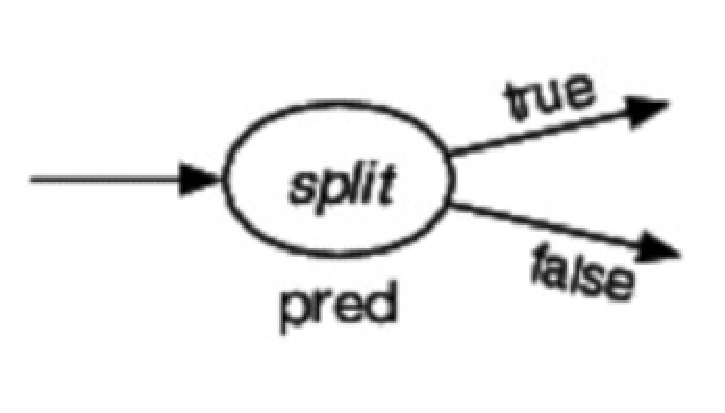
\includegraphics[width=8cm]{fig_06_003.eps}


\texttt{core.async}の \texttt{split} 関数は、1つのチャネルを受け取り、述語の真偽に基づいてトラフィックを2つの出力チャネルに分割します。これは図に示すとおりです。

例えば、\texttt{split} はストリームから無効なメッセージを分割し、別のプロセスに送って処理するのに適した方法です。


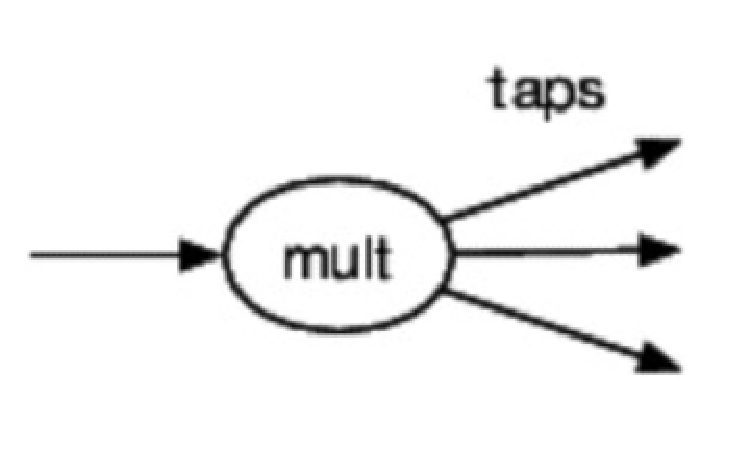
\includegraphics[width=8cm]{fig_06_004.eps}

\texttt{core.async}の \texttt{mult} 抽象化は、入力チャネルを受け取り、それを複数の出力チャネルに乗算します。

入力チャネルから項目が読み込まれると、次の値に移る前にすべての出力チャネルに供給されます。タップは \texttt{tap} 関数で \texttt{mult} に追加され(\texttt{untap} で削除され)ます。タップが閉じていることが判明した場合、そのタップは mult から削除されます。

すべてのチャネルが各値を受信する必要があるため、1つの遅いタップが \texttt{mult} を停止させる可能性があります。そこで、別のバッファリング戦略を使用することが有効です。例えば、パイプラインの特定の部分の出力ストリームをタップしてログにシャントし、何が起こっているかを覗き見ることができるようにしたいとします。

この関数は、入力と出力のチャネルを接続します( \texttt{pipe} で行ったことと同様です)が、返されるログのタップもインストールします。


\begin{lstlisting}[numbers=none]
(defn connect-and-tap
  "入力と出力を接続し、その間を流れるチャネルロギングデータを返します。"
  [input output]
  (let [m (mult input)
       log (chan (dropping-buffer 100))]
    (tap m output)
    (tap m log)
    log))
\end{lstlisting}

 % Connecting Components with Channels
\section{コンポーネントを実装する}

さて、コンポーネントをどのように呼び出し、接続するかという観点から見てきましたが、次はAPIの背後にある機能をどのように実装するかという内部事情に目を向ける必要があります。

ほとんどのコンポーネントはある種の状態を保持しており、呼び出し側がこの状態を更新したり、状態に依存する機能を呼び出したりすることができます。これまで学んできた状態のメカニズム( atom 、 ref 、 agent )は多くの方法で使用することができ、特に状態の粒度をどのように選択するかを検討します。

また、コンポーネントのライフサイクル全体についても考慮する必要があります。コンポーネントは、構成データと依存関係で構築され、内部状態や外部システムとの接続を初期化する必要があるかもしれません。コンポーネントが構築されたら、各コンポーネントを停止するためのパスも用意しておくとよいでしょう。これは、開発中にREPLで簡単に起動・停止できるようなシステムを構築するために重要です。この2つについて、さらに詳しく見ていきましょう。

まず、各コンポーネント内の状態の粒度について見ていきます。

\subsection{状態の粒度}

コンポーネントはしばしば、コンポーネントの寿命の間に変更される可能性のある実行時の状態を持っています。これはコンポーネントが管理するデータであったり、 データベース接続のような内部ステートフルリソースハンドルであったり、 あるいは動的な設定値であったりします。実行状態の初期値は設定の一部として渡されることもありますが、多くの場合、内部で構築されたり、時間の経過とともに構築されたりします。

コンポーネント内に状態を保持する場合、ステートフルなコンテナ(通常は atom か ref )を使用する必要があります。どちらを使うか、そしてステートの粒度を選択する必要がある。

主な決定要因は、必要な調整のレベルです。 atom はより単純だが、複数のステート間で調整することができない。 ref はより複雑だが、協調をサポートする。しかし、別の見方をすると、調整が必要な2つの状態の断片を1つの atom の下に持ってきて、再び1つの更新関数で対応できるようにすることも可能である。

口座のインデックスと顧客のインデックスという2種類の状態を管理する必要があるコンポーネントを考えてみましょう。これらは2つの atom として維持することができる。

\begin{lstlisting}[numbers=none]
(defrecord CustomerAccounts [accounts customers])

(defn make-customer-accounts []
  (map->CustomerAccounts {:accounts (atom {})
                          :customers (atom {})}))
\end{lstlisting}

あるいは、アカウントとカスタマーの両方でトランザクション的に変更が必要なケースであれば、 ref を使うことも可能でした。


\begin{lstlisting}[numbers=none]
(defrecord CustomerAccounts [accounts customers])

(defn make-customer-accounts []
  (map->CustomerAccounts {:accounts (ref {})
                          :customers (ref {})}))
\end{lstlisting}

ref を使用すると、コンポーネントの状態との相互作用にトランザクションを巻き付ける必要があります。その代わりに、状態の粒度を大きくして、1つの atom 内にアカウントと顧客の両方を包含することができるかもしれません。

\begin{lstlisting}[numbers=none]
(defrecord CustomerAccounts [state])

(defn make-customer-accounts []
  (map->CustomerAccounts (atom {:accounts {}
                                :customers {}})))
\end{lstlisting}

Clojureの atom は高速なので、更新関数が小さいことを前提に、その内部で粗視化された状態を使うことができる場合が多いのです。

逆に、口座や顧客を桁ごとに分割したり、名前ごとに分割してセグメントごとにrefを作成するなど、粒度をより細かくすることも可能です。コンポーネントのトップレベルの機能は影響を受けますが、エンティティレベルのデータや関数はシンプルでステートレス、そしてどのようなアプローチにも完全に再利用可能であるべきです。

\subsection{構成}

コンポーネントを実装する際には、起動時や継続的に使用するために必要な情報を保持する必要があります。コンポーネントは、構成、依存関係、実行時の状態という3つの主要な情報を必要とします。

設定データは、コンポーネントの外部で取得したり構築したりします (設定データの管理方法については、第7章 アプリケーションの構成で説明します)。作成時にコンポーネントに渡され、コンポーネントの起動時またはそれ以降に使用することができます。設定情報の一般的な使用例としては、外部リソース (データベースやメッセージシステムなど) への接続パラメータがあります。

コンポーネントを作成する際に、各設定値を個別のパラメータとして渡すことができます。

\begin{lstlisting}[numbers=none]
(defn new-component [db-url user password] ...)
\end{lstlisting}

しかし、設定データはシステムの開発に伴って変化することが多いので、設定データは必要に応じて進化できるパッケージ(マップやレコード)として渡すのがよい。

\begin{lstlisting}[numbers=none]
(defn new-component [{:keys [db-url user password]}] ...)
\end{lstlisting}

設定データだけでなく、コンポーネントが他のコンポーネントを参照する必要がある場合も多い。例えば、ナレッジエンジンコンポーネントは、設定データに加えて、データフィードコンポーネントへのアクセスを必要とする場合があります。

\begin{lstlisting}[numbers=none]
(defn new-knowledge-engine [config feed] ...)
\end{lstlisting}

しかし、あるコンポーネントを依存関係として他のコンポーネントに直接渡すよりも、それらの間にチャネルを配置することによってそれらを切り離す方が理にかなっている場合もあります。この場合、リモートコンポーネントではなく、チャネルが依存関係として扱われます。コンポーネントの接続方法を考えると、これはコンポーネントの組み立てに多くの選択肢を与えることになります。

コンポーネントには、設定、他のコンポーネントやチャネルとの依存関係、内部のランタイムの状態を保存する場所が必要です。レコードは、コンポーネントの動作を定義するプロトコルを実装するのが一般的であるため、これに最適な選択肢である。

次に、コンポーネントの状態が作成されるコンストラクションを含む、コンポーネントのライフサイクルを見ていきます。

\subsection{ライフサイクル}

ほとんどのコンポーネントのライフサイクルは単純である。最も重要なイベントは、構築、コンポーネントの開始、およびコンポーネントの停止です。

例えば、先ほどのルールベースの知識エンジンと、そのコンポーネントをどのように構築するかを考えてみましょう。議論のために、知識エンジンは受信メッセージのストリームを受け取り、ルールに従ってそれを修正し、他のコンポーネントに送信する役割を担っていることも考えてみましょう。

\begin{lstlisting}[numbers=none]
(defrecord KnowledgeEngine
  [config ;; map of config info
   ch-in ;; channel to receive messages
   ch-out ;; channel to post messages
   rules ;; state - current rule set
   active]) ;; state - true if active

(defn make-knowledge-engine
  [config ch-in ch-out rule-set]
  (->KnowledgeEngine config ch-in ch-out
          (atom rule-set) (atom false)))

(defn start-knowledge-engine
  [{:keys (ch-in ch-out rules active) :as ke}]
  (reset! active true)
  (go-loop [request (<! ch-in)
            response (fire-rules ke request)]
    (>! ch-out response)
    (when @active (recur)))
  ke)

(defn stop-knowledge-engine
  [{:keys (ch-out active) :as ke}]
  (reset! active false) ;; exit go loop
  (async/close! ch-out) ;; stop producing
  ke)
\end{lstlisting}

コンポーネントはしばしばステートフルフィールドに初期値を設定したり、その他のタスクを実行する必要があるため、通常、コンポーネントインスタンスを作成するためのカスタム関数を提供することになります。ここでは、 \texttt{make-knowledge-engine} 関数は、知識エンジンの現在のルールの状態を保持するアトムを含む、コンポーネントのインスタンスを構築します。

静的な構成は、しばしばアプリケーションの進化に伴う変更の原因となります。この進化を計画するには、静的構成を一連の位置づけの構成パラメータとしてではなく、マップとして捉えるのが最適です。これにより、頻繁に変更される設定値を、既存のコードを壊すことなく変更することができます。

\texttt{start-knowledge-engine} 関数は、受信した要求チャネルの処理を開始するためにコンポーネントをアクティブにします。軽量なgoブロックが作成され、コンポーネントの寿命まで生き続け、 \texttt{ch-in} からメッセージを抽出し、ルールを介してそれを処理し、 \texttt{ch-out} にそれを投稿します。ステートフルアクティブフラグは、ゴーブロックが継続すべきかどうかを決定するために使用されます。

\texttt{stop-knowledge-engine} 関数は \texttt{active} フラグを \texttt{false} に設定し、goブロックのループを停止させることができる。 \texttt{stop} 関数はまた、これ以上メッセージが生成されないため、出力チャネルを閉じます。入力チャネルは閉じません。その代わり、コンポーネントが停止したときに、入力チャネルのオーナーがそのチャネルをクローズする必要があります。これは \texttt{core.async} プログラムでよくある慣習です。




 % Implementing Components
\section{まとめ}

コンポーネントは、アプリケーションの実際の機能を確立する、より大きなコードの単位を構築するための手段です。コンポーネントは構造を提供し、チームが作業を分担するために使用できるコードの有意義なサブユニットを作成します。

まず、コンポーネントの外部API(関数、非同期呼び出し、チャンネルによるイベントストリーム)を設計する方法と、 core.async を使用してこれらのコンポーネントを接続する方法について見ていきました。

また、各コンポーネントの設定データ、依存関係、内部状態、コンポーネントのライフサイクルを考慮した実装方法についても見てきました。

次に、システムを組み立てるための全体像を探ります。アプリケーションの設定データをどのように管理し、コンポーネントに提供するか、コンポーネントをどのようにインスタンス化して接続するか、システムのエントリポイントをどのように提供するか、について見ていきます。 % Wrapping Up